LSTM – là 1 dạng đặc biệt của mô hình RNN (Recurrent Neural Network), có khả năng học được các phụ thuộc. Phương pháp chính của mô hình LSTM là trạng thái tế bào (cell state), nó tương tự như 1 băng truyền chạy xuyên suốt tất cả các mắt xích và tương tác tuyến tính với các mắt xích đó vì vậy mà các thông tin dễ dàng truyền đi thông suốt mà không sợ bị thay đổi. LSTM sở hữu khả năng chọn lọc thông tin quan trọng bằng cách loại bỏ hoặc thêm vào trạng thái (state) của nó. Quá trình này được kiểm soát bởi các cấu trúc được gọi là cổng (gate). Mỗi cổng hoạt động như một bộ lọc thông tin, quyết định lượng thông tin được phép đi qua. Cụ thể, cổng bao gồm một lớp mạng sigmoid, tạo ra một giá trị trong khoảng từ 0 đến 1, đại diện cho tỷ lệ thông tin được truyền qua. Giá trị 0 nghĩa là không có thông tin nào được truyền qua, trong khi giá trị 1 cho phép tất cả thông tin đi qua. LSTM sử dụng ba cổng như vậy để quản lý và điều chỉnh trạng thái của tế bào: cổng quên (forget gate), cổng vào (input gate) và cổng ra (output gate).

\begin{figure}[htbp]
\centerline{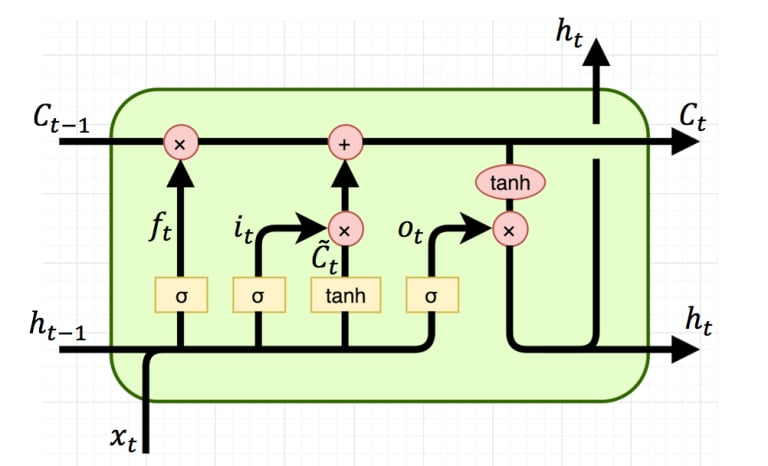
\includegraphics[width=0.4\textwidth]{img/LSTM.jpg}}
\caption{Kiến trúc LMST.}
\label{fig}
\end{figure}